In diesem Experiment ist der Platz für Bewegungen sehr beschränkt. Zwölf Felder sind von Agenten belegt und lediglich neun sind frei. 

\textbf{Aufbau des Experiments}
\begin{figure}[H]
    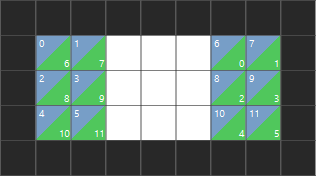
\includegraphics[height=40mm]{images/6vs6_tight.png}
    \centering
    \caption{Aufbau für die enge Vorbeifahrt zweier Gruppen, bestehend aus jeweils sechs Agenten}
    \label{fig:6x6Eng}
\end{figure}
Die Karte für dieses Experiment ist sieben mal drei Felder groß. Es stehen sich zwei Gruppen aus jeweils sechs Agenten gegenüber. Wie in Abbildung \ref{fig:6x6Eng} zu erkennen, befindet sich zwischen den beiden Gruppen ein Block aus drei mal drei freien Feldern.